\documentclass[12pt,a4paper]{article}
\usepackage[utf8]{inputenc}
\usepackage[brazil]{babel}
\usepackage{graphicx}
\usepackage{amssymb, amsfonts, amsmath}
\usepackage{color}
\usepackage{float}
\usepackage{enumerate}
%\usepackage{subfigure}
\usepackage[top=2.5cm, bottom=2.5cm, left=1.25cm, right=1.25cm]{geometry}

\newcommand{\sen}{\,\textrm{sen}\,}
\newcommand{\tg}{\,\textrm{tg}\,}

\begin{document}
\pagestyle{empty}

\begin{center}
\begin{tabular}{ccc}
\begin{tabular}{c}
\includegraphics[scale=0.25]{../../biblioteca/imagem/brasao-de-armas-brasil} \\
\end{tabular} & 
\begin{tabular}{c}
Ministério da Educação \\
Universidade Federal dos Vales do Jequitinhonha e Mucuri \\
Faculdade de Ciências Sociais, Aplicadas e Exatas - FACSAE \\
Departamento de Ciências Exatas - DCEX \\
Disciplina: Cálculo Numérico\\
Prof.: Luiz C. M. de Aquino\\
\end{tabular} &
\begin{tabular}{c}
\includegraphics[scale=0.25]{../../biblioteca/imagem/logo-ufvjm} \\
\end{tabular}
\end{tabular}
\end{center}

\begin{center}
 \textbf{Lista de Exercícios IV}
\end{center}

\begin{flushleft}
 \textbf{Observação}

 Nesta lista de exercícios, todos os sistemas de equações devem ser resolvidos por Eliminação Gaussiana.
\end{flushleft}

\begin{enumerate}
  \item Resolva o sistema de equações:
  $$\begin{cases}10x + 2y + z = 23 \\ 2x + y + 5z = 19 \\ x + 5y + z = 20 \end{cases}$$

  \item Uma empresa de transporte possui três tipos de caixa: $A$, $B$ e
$C$. Cada caixa pode transportar simultaneamente três tipos de produtos
($X$, $Y$ e $Z$) na quantidade descrita pela tabela abaixo. Com
base nessas informações, quantas caixas de cada tipo são necessárias
para transportar $590$ unidades de $X$, $255$ de $Y$ e $480$
de $Z$? \\
\begin{table}[H]
\centering%
\begin{tabular}{|c|c|c|c|}
\cline{2-4} 
\multicolumn{1}{c|}{} & $X$ & $Y$ & $Z$\\
\hline 
$A$ & 10 & 5 & 4\\
\hline 
$B$ & 6 & 3 & 8\\
\hline 
$C$ & 20 & 8 & 16\\
\hline 
\end{tabular}
\end{table}

  \item Um fabricante de móveis produz cadeiras, mesinhas de centro e mesas
de jantar. Cada cadeira leva 10 minutos para ser lixada, 6 minutos
para ser tingida e 12 minutos para ser envernizada. Cada mesinha de
centro leva 12 minutos para ser lixada, 8 minutos para ser tingida
e 12 minutos para ser envernizada. Cada mesa de jantar leva 15 minutos
para ser lixada, 12 minutos para ser tingida e 18 minutos para ser
envernizada. A bancada para lixar fica disponível 1.340 minutos por
semana, a bancada para tingir 940 minutos por semana e a bancada para
envernizar 1.560 minutos por semana. Quantos móveis devem ser fabricados
(por semana) de cada tipo para que as bancadas sejam plenamente utilizadas?

 \item Considere o problema do circuito hidráulico mostrado na Figura~\ref{fig:tub}. Este sistema está alimentado por um reservatório 
cuja a pressão é mantida constante e igual a $P_r = 10$. As saídas das tubulações desembocam na atmosfera, onde a pressão é 
considerada nula (isto é, $P_a = 0$). Deste modo, a vazão $Q_i$ da $i$-ésima tubulação depende da diferença de pressão $\Delta P_i$ 
de tal modo que $$Q_i = K_iL_i\Delta P_i,$$ onde $K_i$ é a resistência hidráulica e $L_i$ o comprimento da tubulação. Por exemplo, para a 
tubulação $8$ temos que $Q_8 = K_8L_8\Delta P_8$, sendo que $\Delta P_8 = P_1 - P_4$ (ou seja, a pressão que ``entra'' na tubulação pela 
bifurcação $1$ menos a pressão que ``sai'' da tubulação pela bifurcação $4$). Por outro lado, sabe-se que em cada bifurcação a soma das vazões 
deve ser nula. Por exemplo, na bifurcação $4$ temos que $Q_8 - Q_6 - Q_7 = 0$ (aqui note que a vazão que ``entra'' na bifurcação é considerada positiva, 
enquanto que a que ``sai'' é considerada negativa). Considerando essas informações e os dados da Tabela~\ref{tab:dados}, determine as vazões em cada tubulação e as pressões 
em cada bifurcação.

\begin{figure}[!htb]
 \centering
 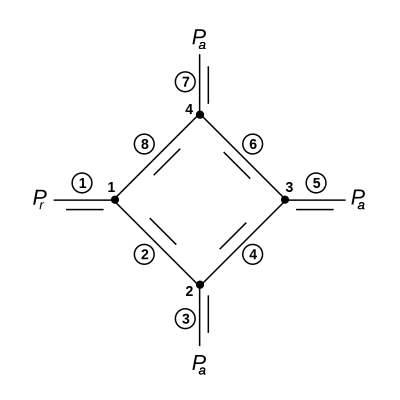
\includegraphics[scale=0.75]{imagem/Tubulacao.png}
 \caption{Esquema do circuito hidráulico.}
 \label{fig:tub}
\end{figure}

\begin{table}[!htb]
 \centering
 \begin{tabular}{c|c|c}
  Tubulação $i$ & $K_i$ & $L_i$ \\ \hline
  1 & 0,02 & 1,0 \\ \hline
  2 & 0,005 & 2,0 \\ \hline
  3 & 0,085 & 0,5 \\ \hline
  4 & 0,02 & 1,0 \\ \hline
  5 & 0,075 & 0,5 \\ \hline
  6 & 0,085 & 0,5 \\ \hline
  7 & 0,015 & 2,0 \\ \hline
  8 & 0,01 & 1,0 
 \end{tabular}
 \caption{Resistência hidráulica e comprimento das tubulações.}
 \label{tab:dados}
\end{table}
 
\end{enumerate}

\begin{center}
\textbf{Gabarito}
\end{center} 
\textbf{[1]} $x = 1,4$, $y = 3,2$ e $z = 2,6$.
\textbf{[2]} $A=10$, $B=15$ e $C=20$. 
\textbf{[3]} $50$ cadeiras, $20$ mesinhas de centro e $40$ mesas de jantar. 
\textbf{[4]} $P_1 = 5,47246730738932$, $P_2 = 0,919331967858831$, $P_3 = 0,596344729793603$, $P_4 = 0,970537261698440$. 
$Q_1 = 0,0905506538522137$, $Q_2 = 0,0455313533953049$, $Q_3 = 0,0390716086340003$, $Q_4 = 0,00645974476130455$, 
$Q_5 = 0,0223629273672601$, \\ $Q_6 = 0,0159031826059556$, $Q_7 = 0,0291161178509532$, $Q_8 = 0,0450193004569088$.
\end{document}
